\documentclass[12pt, a4paper]{article}

%%=============================================================
%% PACKAGES
%%=============================================================
\usepackage[indonesian]{babel}
\usepackage[utf8]{inputenc}
\usepackage[T1]{fontenc}
\usepackage{setspace}
\usepackage{graphicx}
\graphicspath{{../Project/gambar/}{gambar/}}
\usepackage{float}
\usepackage{indentfirst}
\setlength\parindent{1cm}
\usepackage{pslatex}
\usepackage{tabularx}
\usepackage{multirow}
\usepackage{colortbl}
\usepackage{xcolor}
\usepackage{amsmath}
\usepackage{amssymb}
\usepackage{enumitem}
\usepackage{longtable}
\usepackage{booktabs}
\usepackage{titlesec}
\usepackage{caption}
\usepackage{geometry}
\usepackage{fancyhdr}
\usepackage[hidelinks]{hyperref}

%%=============================================================
%% LAYOUT
%%=============================================================
\geometry{a4paper, left=4cm, top=4cm, right=3cm, bottom=3cm}

\setlength{\headheight}{14.5pt}
\pagestyle{fancy}
\fancyhf{}
\rhead{\thepage}
\renewcommand{\headrulewidth}{0pt}
\renewcommand{\footrulewidth}{0pt}

\setstretch{1.5}

\tolerance=1
\emergencystretch=\maxdimen
\hyphenpenalty=10000
\hbadness=10000

%%=============================================================
%% SECTION FORMAT
%%=============================================================
\setlist{nosep}

\renewcommand{\thesection}{\Alph{section}.\hspace{0.18cm}}
\renewcommand{\thesubsection}{\arabic{subsection}.}

\titleformat{\section}{\fontsize{12}{14}\bfseries}{\thesection}{0.4cm}{}
\titleformat{\subsection}{\fontsize{12}{14}\bfseries}{\thesubsection}{0.675cm}{}
\titlespacing*{\section}{0pt}{10pt}{0pt}
\titlespacing*{\subsection}{0pt}{10pt}{0pt}

\captionsetup[figure]{labelsep=space, labelfont=bf, format=plain}
\captionsetup[table]{labelsep=space, labelfont=bf, format=plain}

%%=============================================================
%% GANTT CHART HELPERS
%%=============================================================
\definecolor{jadwal}{gray}{0.65}
\newcommand{\G}{\cellcolor{jadwal}}
\newcolumntype{W}{>{\centering\arraybackslash}m{0.36cm}}

%%=============================================================
%% DOCUMENT
%%=============================================================
\begin{document}

%%-------------------------------------------------------------
%% HALAMAN JUDUL
%%-------------------------------------------------------------
\begin{titlepage}
\thispagestyle{empty}
\setstretch{1.0}
\begin{center}

{\fontsize{14}{16}\selectfont\bfseries PROPOSAL PENELITIAN SKRIPSI}

\vspace{1.5cm}

{\fontsize{14}{16}\selectfont\bfseries
RANCANG BANGUN APLIKASI \textit{POINT OF SALE} DENGAN FITUR\\[4pt]
PREDIKSI PENJUALAN HARIAN MENGGUNAKAN METODE\\[4pt]
\textit{LONG SHORT-TERM MEMORY} (LSTM)}

\vspace{2.5cm}


\includegraphics[width=3.5cm]{logo-pnl-skripsi}

\vspace{2.5cm}

Disusun oleh:\\[0.5cm]
{\bfseries MUHAMMAD KHOLIS\\[4pt]
2022573010098}

\vfill

{\bfseries
TEKNOLOGI INFORMASI KOMPUTER\\[4pt]
TEKNIK INFORMATIKA\\[4pt]
POLITEKNIK NEGERI LHOKSEUMAWE\\[4pt]
TAHUN 2026}

\end{center}
\end{titlepage}

%%-------------------------------------------------------------
%% HALAMAN PERSETUJUAN
%%-------------------------------------------------------------
\newpage
\thispagestyle{empty}
\setstretch{1.5}

\begin{center}
{\fontsize{14}{16}\selectfont\bfseries HALAMAN PERSETUJUAN}
\end{center}

\vspace{0.4cm}

\begin{center}
\textbf{RANCANG BANGUN APLIKASI \textit{POINT OF SALE} DENGAN FITUR PREDIKSI\\
PENJUALAN HARIAN MENGGUNAKAN METODE \textit{LONG SHORT-TERM}\\
\textit{MEMORY} (LSTM)}
\end{center}

\vspace{0.5cm}

\noindent Dipersiapkan dan Disusun oleh\\[0.2cm]
\indent\textbf{MUHAMMAD KHOLIS}\\
\indent\textbf{2022573010098}

\vspace{0.5cm}

\noindent Telah disetujui oleh Tim Dosen Pembimbing Penelitian Skripsi
pada tanggal 12 Mei 2026

\vspace{0.8cm}
\noindent Buketrata, 12 Mei 2026

\vspace{1cm}

\noindent
\begin{tabular}{p{0.44\textwidth}p{0.08\textwidth}p{0.38\textwidth}}
Mengetahui: & & Ketua Pengusul, \\
Ketua Prodi Teknik Informatika & & \\[3.2cm]
\textbf{M. Khadafi, S.T., M.T.} & & \textbf{Muhammad Kholis} \\
NIP. 197507182002121004 & & NIM. 2022573010098 \\
\end{tabular}

\vspace{1.5cm}

\noindent Menyetujui,\\
Ketua Jurusan Teknologi Informasi \& Komputer

\vspace{3.2cm}

\noindent\textbf{Salahuddin, S.T., M.Cs.}\\
NIP. 197404242002121001

%%-------------------------------------------------------------
%% ISI PROPOSAL
%%-------------------------------------------------------------
\newpage
\pagenumbering{arabic}
\setcounter{page}{1}

%%-------------------------------------------------------------
\section{Latar Belakang Masalah}

Fenomena digitalisasi di Indonesia telah mengalami akselerasi yang signifikan dalam lima tahun terakhir, namun adopsi teknologi di tingkat UMKM lokal sering kali terbentur pada kompleksitas penggunaan dan biaya infrastruktur yang tinggi. Di Kota Lhokseumawe, program pembinaan pemerintah melalui Dinas Perdagangan, Koperasi, dan UKM telah berupaya meningkatkan kapasitas manajerial pelaku usaha, namun efektivitasnya sering kali terhambat oleh kurangnya alat bantu yang mampu memberikan data secara \textit{real-time} untuk pengambilan keputusan strategis. Pencatatan transaksi manual yang masih mendominasi menyebabkan data sejarah penjualan tidak terorganisir dengan baik, sehingga sulit untuk mengidentifikasi pola musiman atau tren permintaan konsumen.

Sifat data penjualan ritel yang merupakan deret waktu (\textit{time series}) mengandung kompleksitas non-linier yang dipengaruhi oleh berbagai faktor eksternal seperti hari libur, hari gajian, hingga fluktuasi cuaca. Model statistik tradisional seperti ARIMA sering kali gagal menangkap hubungan jangka panjang dalam data yang sangat fluktuatif ini. Oleh karena itu, penerapan algoritma \textit{deep learning} seperti LSTM menjadi relevan karena arsitekturnya yang mampu mempertahankan memori jangka panjang melalui mekanisme gerbang (\textit{gates}) yang kompleks. Pemanfaatan VPS untuk komputasi berat model LSTM di belakang layar memastikan bahwa aplikasi \textit{mobile} tetap ringan dan responsif saat digunakan di perangkat dengan spesifikasi terbatas.

Pentingnya penelitian ini juga didorong oleh tren industri 4.0 yang menuntut efisiensi operasional melalui pendekatan \textit{data-driven decision making}. Dengan adanya fitur prediksi, pelaku UMKM dapat melakukan optimasi stok secara otomatis, mengurangi risiko pemborosan modal, dan meningkatkan efisiensi rantai pasok secara keseluruhan. Fokus pada UMKM di Lhokseumawe memberikan dimensi studi kasus yang spesifik, memungkinkan pengembangan solusi yang kontekstual dengan kebutuhan lokal namun tetap berbasis pada standar teknologi global.

%%-------------------------------------------------------------
\section{Rumusan Masalah}

Berdasarkan uraian latar belakang di atas, identifikasi masalah yang akan dikaji dalam penelitian ini dirumuskan sebagai berikut:
\begin{enumerate}[leftmargin=1.5\parindent]
    \item Bagaimana merancang arsitektur aplikasi \textit{Point of Sale} berbasis \textit{mobile} menggunakan \textit{framework} Flutter yang mampu mengintegrasikan operasional kasir dengan modul prediksi penjualan secara \textit{real-time}?
    \item Bagaimana mekanisme sinkronisasi data antara aplikasi \textit{mobile}, basis data Supabase, dan model LSTM yang dijalankan pada \textit{Virtual Private Server} untuk memastikan akurasi data pelatihan?
    \item Berapa tingkat efektivitas dan akurasi model LSTM dalam memprediksi volume penjualan harian pada UMKM di Lhokseumawe jika diukur dengan metrik \textit{Mean Absolute Percentage Error} (MAPE) dan \textit{Root Mean Squared Error} (RMSE)?
    \item Sejauh mana aplikasi POS ini dapat membantu meminimalisir kesalahan manajemen stok barang bagi pemilik usaha melalui fitur estimasi stok otomatis?
\end{enumerate}

%%-------------------------------------------------------------
\section{Batasan Masalah}

Penelitian ini dibatasi oleh beberapa parameter utama untuk memastikan fokus dan kedalaman hasil:
\begin{enumerate}[leftmargin=1.5\parindent]
    \item Aplikasi dikembangkan khusus untuk platform Android menggunakan bahasa pemrograman Dart dan \textit{framework} Flutter.
    \item Basis data yang digunakan adalah Supabase dengan skema relasional untuk menyimpan data produk, transaksi, dan akun pengguna.
    \item Implementasi algoritma prediksi terbatas pada metode LSTM tanpa melakukan perbandingan mendalam dengan arsitektur lain seperti GRU atau Bi-LSTM dalam tahap produksi.
    \item Data uji yang digunakan bersumber dari data transaksi riil UMKM mitra di Lhokseumawe dengan periode minimal satu tahun atau setidaknya mencakup siklus musiman tahunan.
    \item Variabel input untuk prediksi hanya mencakup data historis volume penjualan tanpa menyertakan variabel eksternal seperti suhu, berita ekonomi, atau tren media sosial.
\end{enumerate}

%%-------------------------------------------------------------
\section{Tujuan Penelitian}

Kegiatan penelitian ini bertujuan untuk:
\begin{enumerate}[leftmargin=1.5\parindent]
    \item Membangun aplikasi POS \textit{mobile} yang fungsional untuk memudahkan UMKM dalam mencatat penjualan, pembelian, dan inventaris secara terpusat.
    \item Mengembangkan model \textit{deep learning} LSTM yang mampu mengekstraksi pola penjualan dari data historis transaksi UMKM lokal.
    \item Mengintegrasikan model prediksi ke dalam dasbor aplikasi \textit{mobile} sehingga pemilik usaha mendapatkan rekomendasi jumlah pengadaan stok secara visual.
    \item Mengevaluasi performa sistem dari sisi kegunaan (\textit{usability}) dan akurasi komputasi untuk memastikan solusi dapat diandalkan dalam lingkungan bisnis nyata.
\end{enumerate}

%%-------------------------------------------------------------
\section{Manfaat Penelitian}

Hasil penelitian ini diharapkan memberikan manfaat yang luas pada berbagai pemangku kepentingan:
\begin{enumerate}[leftmargin=1.5\parindent]
    \item \textbf{Bagi Pelaku UMKM:} Memberikan alat bantu teknologi yang terjangkau untuk meningkatkan produktivitas, mengurangi risiko stok kosong, dan meningkatkan kualitas layanan kepada konsumen.
    \item \textbf{Bagi Peneliti:} Memperkaya khazanah keilmuan mengenai aplikasi praktis kecerdasan buatan pada perangkat \textit{mobile} dan memberikan data empiris mengenai perilaku konsumsi masyarakat di wilayah Aceh.
    \item \textbf{Bagi Institusi (Politeknik Negeri Lhokseumawe):} Menjadi bukti kontribusi nyata akademisi dalam menyelesaikan permasalahan ekonomi lokal melalui inovasi teknologi informatika.
\end{enumerate}

%%-------------------------------------------------------------
\section{Tinjauan Pustaka}

Kajian literatur dalam penelitian ini mencakup perbandingan antara berbagai metode peramalan penjualan dan implementasi sistem informasi manajemen ritel. Perkembangan teknologi jaringan saraf tiruan telah membawa perubahan besar dalam efisiensi peramalan bisnis.

\subsection{Perbandingan Metode Peramalan Penjualan}

Berbagai penelitian terdahulu menunjukkan keunggulan metode \textit{deep learning} dibandingkan model statistik klasik. Dalam studi peramalan penjualan produk aerosol, ditemukan bahwa LSTM memberikan performa terbaik dengan nilai MAPE sebesar 10,76\%, mengungguli ARIMA (11,23\%) dan GRU (11,47\%) dalam menangkap tren jangka panjang. Hal ini diperkuat oleh penelitian pada koperasi sekolah di Malang yang mencapai akurasi 88,19\% melalui arsitektur LSTM hibrida untuk produk makanan yang memiliki volatilitas tinggi.

\begin{table}[H]
\setstretch{1.2}
\centering
\caption{Perbandingan Metode Peramalan Penjualan}
\label{tab:perbandingan}
\begin{tabularx}{\textwidth}{|l|X|X|X|}
\hline
\textbf{Metrik Evaluasi} & \textbf{LSTM (Deep Learning)} & \textbf{ARIMA (Statistik)} & \textbf{GRU (Gated Unit)} \\
\hline
Kapasitas Data & Sangat baik untuk dataset besar & Terbatas pada data linear & Efisien untuk dataset menengah \\
\hline
Waktu Pelatihan & Relatif lama karena kompleksitas gerbang & Cepat namun kaku & Lebih cepat dari LSTM \\
\hline
Akurasi (MAPE) & Umumnya $<$ 12\% pada data ritel & Berkisar 20--25\% & Mendekati LSTM \\
\hline
Kebutuhan Memori & Tinggi & Rendah & Sedang \\
\hline
\end{tabularx}
\end{table}

Penelitian lain di bidang peramalan penjualan laptop mengategorikan produk berdasarkan rentang harga dan menemukan bahwa LSTM sangat akurat untuk kategori harga menengah (\textit{mid-end}) dengan skor R-squared mencapai 0,9890. Keberhasilan ini mengindikasikan bahwa perilaku konsumen pada segmen tertentu lebih mudah dipelajari oleh algoritma jika dataset memiliki kerapatan informasi yang cukup.

\subsection{Implementasi Sistem POS \textit{Mobile}}

Pengembangan aplikasi POS berbasis Android telah banyak dieksplorasi menggunakan berbagai teknologi. Penggunaan Firebase sebagai basis data \textit{real-time} sering menjadi pilihan utama bagi pengembang karena kemudahan sinkronisasi, namun penelitian terbaru mulai beralih ke Supabase atau integrasi API khusus untuk fleksibilitas manajemen data yang lebih besar. \textit{Framework} Flutter terbukti efektif dalam membangun antarmuka yang responsif dan memudahkan integrasi fitur-fitur modern seperti pembayaran QRIS.

Sistem POS yang dirancang untuk UMKM memerlukan pendekatan yang berbeda dibandingkan sistem ritel besar. Fokus utama harus terletak pada kesederhanaan alur kerja kasir dan kecepatan proses transaksi. Penelitian oleh Rangga Gelar Guntara (2022) menekankan bahwa penggunaan \textit{cloud computing} pada aplikasi POS \textit{mobile} secara signifikan meningkatkan fleksibilitas pemilik usaha dalam memantau bisnis dari mana saja secara \textit{real-time}.

%%-------------------------------------------------------------
\section{Landasan Teori}

Landasan teori menyediakan kerangka konseptual yang mendasari pengembangan sistem, mulai dari teori peramalan hingga arsitektur teknis perangkat lunak.

\subsection{Teori Peramalan (\textit{Forecasting})}

Peramalan penjualan merupakan proyeksi teknis dari permintaan pelanggan potensial untuk periode waktu tertentu berdasarkan asumsi-asumsi yang ditetapkan. Menurut Heizer dan Render, peramalan yang akurat sangat krusial dalam manajemen operasi karena mempengaruhi keputusan strategis di bidang pemasaran, keuangan, dan sumber daya manusia. Terdapat empat prinsip utama dalam peramalan: peramalan jarang sekali sempurna, peramalan jangka pendek biasanya lebih akurat daripada jangka panjang, peramalan agregat lebih akurat daripada peramalan item individu, dan pemilihan metode harus disesuaikan dengan pola data (horizontal, tren, musiman, atau siklis).

Metode kuantitatif dalam peramalan mengandalkan model matematika untuk memproyeksikan data masa lalu ke masa depan. Dalam konteks ritel, tantangan utama adalah menangani variasi musiman, yaitu fluktuasi yang berulang dalam jangka waktu kurang dari satu tahun, seperti lonjakan penjualan menjelang hari raya atau awal bulan.

\subsection{Arsitektur \textit{Long Short-Term Memory} (LSTM)}

LSTM adalah jenis khusus dari \textit{Recurrent Neural Network} (RNN) yang memiliki kemampuan untuk mempelajari ketergantungan jangka panjang dalam urutan data. Arsitektur LSTM dirancang untuk mengatasi masalah \textit{vanishing gradient} yang menghambat RNN standar dalam memproses informasi yang terpisah jauh dalam satu urutan. Komponen inti dari unit LSTM adalah \textit{cell state} (keadaan sel) yang bertindak sebagai jalur informasi utama, serta tiga gerbang fungsional:
\begin{enumerate}[leftmargin=1.5\parindent]
    \item \textbf{\textit{Forget Gate}:} Menggunakan fungsi aktivasi sigmoid untuk menentukan bagian informasi dari status sel sebelumnya yang harus dibuang.
    \item \textbf{\textit{Input Gate}:} Memutuskan informasi baru mana yang akan diperbarui ke dalam status sel melalui kombinasi fungsi sigmoid dan tanh.
    \item \textbf{\textit{Output Gate}:} Menentukan bagian dari status sel yang akan dikeluarkan sebagai \textit{hidden state} untuk langkah waktu berikutnya.
\end{enumerate}

Persamaan matematis sederhana untuk pembaruan status sel $C_t$ dapat dinyatakan sebagai berikut:
\begin{equation}
    C_t = f_t \odot C_{t-1} + i_t \odot \tilde{C}_t
\end{equation}

\noindent Di mana $f_t$ adalah \textit{output} dari \textit{forget gate}, $i_t$ adalah \textit{output} dari \textit{input gate}, dan $\tilde{C}_t$ adalah kandidat nilai baru.

\subsection{\textit{Framework} Flutter dan Bahasa Dart}

Flutter menggunakan mesin grafis Skia untuk merender antarmuka pengguna secara langsung, yang menghasilkan performa tinggi mendekati aplikasi \textit{native}. Bahasa pemrograman Dart yang menyertai Flutter mendukung fitur \textit{Just-In-Time} (JIT) untuk pengembangan cepat dan \textit{Ahead-Of-Time} (AOT) untuk rilis produksi yang efisien. Arsitektur \textit{widget} pada Flutter memungkinkan pengembang untuk membangun komponen antarmuka yang modular dan dapat digunakan kembali, sangat cocok untuk aplikasi POS yang memiliki banyak elemen interaktif.

\subsection{Layanan Supabase dan Integrasi \textit{Cloud}}

Supabase menyediakan lapisan infrastruktur yang matang di atas basis data PostgreSQL, mencakup fitur \textit{real-time subscriptions} yang memungkinkan aplikasi \textit{mobile} menerima pembaruan data secara instan tanpa perlu melakukan \textit{polling} ke server. Penggunaan Supabase dalam penelitian ini memfasilitasi penyimpanan data transaksi dalam jumlah besar yang nantinya akan ditarik oleh modul Python di VPS untuk proses pelatihan model AI.

%%-------------------------------------------------------------
\section{Metode Penelitian}

Metode penelitian mengikuti kerangka kerja pengembangan sistem yang sistematis, didukung oleh teknik pengumpulan data yang valid dan analisis metrik yang ketat.

\subsection{Jenis, Sifat dan Pendekatan Penelitian}

Penelitian ini merupakan jenis penelitian pengembangan (\textit{Research and Development}) dengan pendekatan kuantitatif untuk pengujian model prediksi dan kualitatif untuk analisis kebutuhan pengguna. Model pengembangan yang digunakan adalah \textit{Waterfall}, yang terdiri dari lima tahap utama:
\begin{enumerate}[leftmargin=1.5\parindent]
    \item \textbf{Analisis Kebutuhan:} Mengidentifikasi fitur utama POS (kasir, stok, laporan) dan spesifikasi data untuk kebutuhan LSTM.
    \item \textbf{Desain Sistem:} Membuat arsitektur sistem, skema basis data PostgreSQL, dan rancangan antarmuka (UI/UX).
    \item \textbf{Implementasi:} Melakukan pengkodean \textit{front-end} (Flutter), \textit{back-end} integrasi (Supabase), dan modul AI (Python/TensorFlow).
    \item \textbf{Pengujian:} Melakukan uji coba fungsional menggunakan \textit{Black Box Testing} dan uji akurasi model menggunakan data historis.
    \item \textbf{Pemeliharaan:} Melakukan optimasi parameter model berdasarkan umpan balik penggunaan nyata.
\end{enumerate}

\subsection{Teknik Pengumpulan Data}

Data dikumpulkan melalui tiga saluran utama:
\begin{enumerate}[leftmargin=1.5\parindent]
    \item \textbf{Observasi dan Wawancara:} Dilakukan pada pemilik UMKM di Lhokseumawe untuk memahami proses bisnis dan kendala manajemen stok.
    \item \textbf{Dokumentasi Transaksi:} Mengambil data sejarah penjualan (tanggal, item, jumlah) dari catatan manual atau sistem lama milik mitra UMKM.
    \item \textbf{Studi Pustaka:} Mengkaji referensi jurnal, buku manajemen operasi (Heizer \& Render), dan dokumentasi teknis Flutter/LSTM.
\end{enumerate}

\subsection{Teknik Analisis Data}

Data transaksi yang terkumpul melalui aplikasi POS diproses melalui tahapan berikut sebelum digunakan untuk prediksi:
\begin{enumerate}[leftmargin=1.5\parindent]
    \item \textbf{Pembersihan Data:} Menghapus data duplikat dan mengisi nilai yang kosong menggunakan teknik interpolasi linier untuk memastikan kontinuitas deret waktu.
    \item \textbf{Normalisasi:} Mengubah data volume penjualan ke dalam skala 0 hingga 1 menggunakan MinMaxScaler guna menstabilkan proses pelatihan pada saraf tiruan.
    \item \textbf{Struktur \textit{Supervised Learning}:} Mengubah data sekuensial menjadi format input (X) dan label (y) dengan panjang jendela (\textit{sliding window}) tertentu, misalnya data 14 hari sebelumnya digunakan untuk memprediksi hari berikutnya.
    \item \textbf{Pelatihan Model:} Melatih arsitektur LSTM di VPS menggunakan fungsi aktivasi ReLU pada lapisan tersembunyi dan Adam Optimizer untuk pembaruan bobot.
    \item \textbf{Denormalisasi:} Mengembalikan nilai prediksi ke dalam satuan unit barang untuk ditampilkan pada antarmuka aplikasi.
\end{enumerate}

\subsection{Alur Penelitian}

Alur penelitian ini dirancang secara sistematis untuk membangun sebuah sistem \textit{Point of Sale} (POS) berbasis \textit{mobile} yang dilengkapi dengan fitur prediksi penjualan harian menggunakan metode \textit{Long Short-Term Memory} (LSTM). Tahapan penelitian ini merepresentasikan kerangka kerja pengembangan sistem yang dimulai dari tahap analisis kebutuhan, perancangan, implementasi aplikasi, hingga proses pemodelan dan evaluasi sistem secara menyeluruh.

Sebagaimana diilustrasikan pada Gambar \ref{fig:alur_penelitian}, alur penelitian terbagi menjadi dua fase utama yang saling berkaitan, yaitu Fase Pengembangan dan Implementasi Sistem POS serta Fase Pengembangan Model Prediksi Penjualan.

\begin{figure}[H]
    \centering
    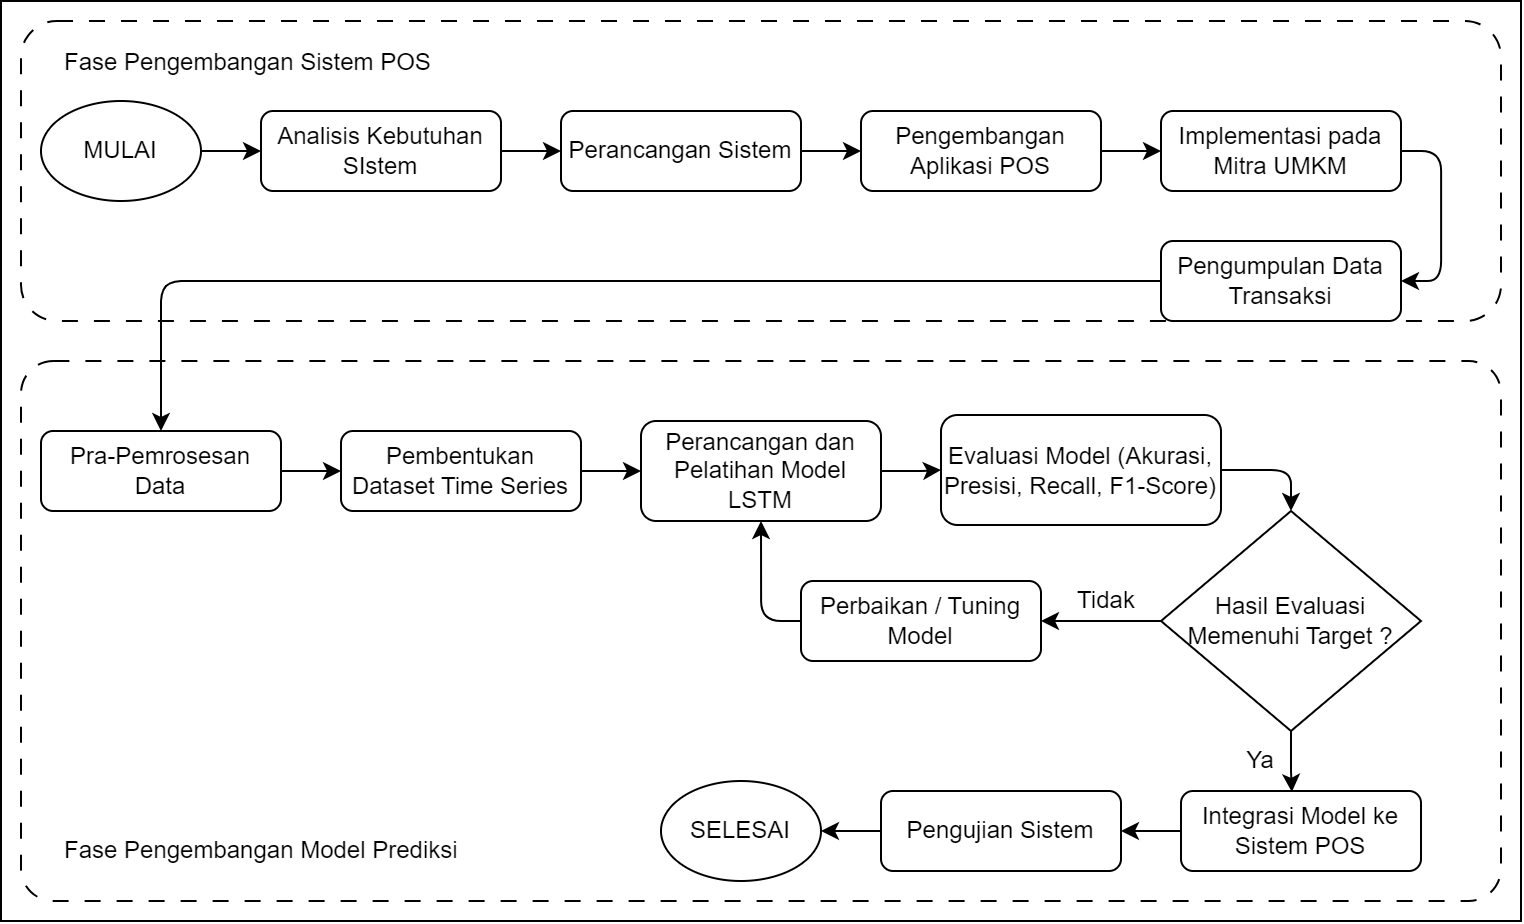
\includegraphics[width=0.85\textwidth]{alur_penelitian}
    \caption{Alur Penelitian}
    \label{fig:alur_penelitian}
\end{figure}

Pada Fase Pengembangan dan Implementasi Sistem POS, penelitian diawali dengan analisis kebutuhan melalui observasi dan identifikasi permasalahan pada mitra UMKM. Selanjutnya dilakukan perancangan sistem meliputi arsitektur aplikasi, desain basis data, serta perancangan UML dan antarmuka pengguna. Setelah tahap perancangan selesai, sistem POS dikembangkan menggunakan Flutter sebagai \textit{frontend}, Supabase sebagai basis data, dan \textit{backend} Python untuk pengolahan data. Aplikasi yang telah dibangun kemudian diimplementasikan pada mitra UMKM untuk digunakan dalam kegiatan transaksi harian. Dari tahap implementasi ini diperoleh data transaksi penjualan aktual yang tersimpan secara otomatis di dalam basis data sistem.

Pada Fase Pengembangan Model Prediksi Penjualan, data transaksi yang telah terkumpul selama periode tertentu selanjutnya melalui tahap pra-pemrosesan (\textit{data preparation}), seperti pembersihan data, agregasi harian, normalisasi, serta pembentukan data runtun waktu (\textit{time series}). Dataset kemudian dibagi menjadi data latih dan data uji untuk proses pemodelan. Model LSTM dilatih menggunakan data latih untuk mempelajari pola penjualan jangka pendek maupun jangka panjang. Setelah proses pelatihan selesai, model diuji menggunakan data uji untuk mengukur tingkat akurasi prediksi dengan metrik evaluasi yang sesuai.

Model prediksi yang telah teruji kemudian diintegrasikan kembali ke dalam sistem POS sehingga aplikasi tidak hanya berfungsi sebagai alat pencatatan transaksi, tetapi juga mampu menampilkan hasil prediksi penjualan harian kepada pengguna. Tahap akhir penelitian dilakukan melalui pengujian fungsional sistem menggunakan metode \textit{black box} serta evaluasi performa model untuk memastikan sistem berjalan sesuai dengan kebutuhan dan tujuan penelitian.

%%-------------------------------------------------------------
\section{Rancangan Sistem}

Perancangan sistem dalam penelitian ini dilakukan menggunakan \textit{Unified Modeling Language} (UML), yang bertujuan untuk memberikan gambaran dan ilustrasi sistem secara jelas dan terstruktur. Pemodelan sistem ini direpresentasikan melalui perancangan \textit{Use Case Diagram}, \textit{Activity Diagram}, serta \textit{User Interface} guna menggambarkan alur proses dan interaksi pengguna dengan sistem.

\subsection{\textit{Use Case Diagram}}

Rancangan sistem pada penelitian ini melibatkan tiga aktor utama, yaitu Admin (Pemilik UMKM), Kasir, dan Pelanggan. \textit{Use Case Diagram} digunakan untuk menggambarkan fungsi-fungsi yang dapat dilakukan oleh masing-masing aktor dalam sistem \textit{Point of Sale} (POS) yang dilengkapi dengan fitur prediksi penjualan harian. Adapun rancangan \textit{use case} pada penelitian ini diilustrasikan pada Gambar \ref{fig:use_case}.

\begin{figure}[H]
    \centering
    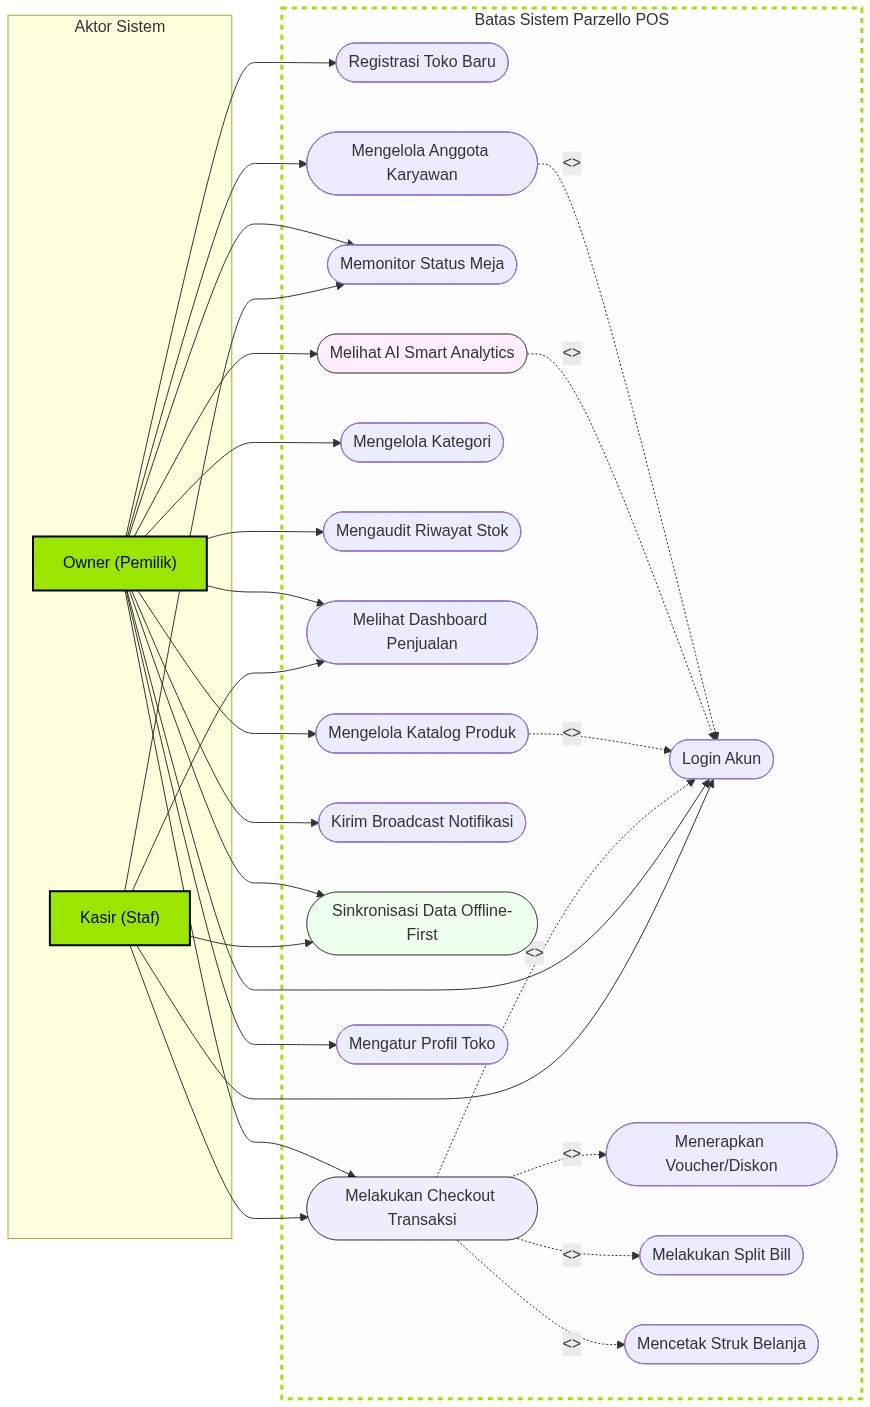
\includegraphics[width=0.85\textwidth]{use_case_diagram}
    \caption{\textit{Use Case Diagram} Sistem POS}
    \label{fig:use_case}
\end{figure}

Gambar \ref{fig:use_case} menggambarkan \textit{use case diagram} pada aplikasi \textit{Point of Sale} (POS) dengan fitur prediksi penjualan harian menggunakan metode LSTM. Penjelasan mengenai aktor dan \textit{use case} pada sistem tersebut dijelaskan sebagai berikut:

\noindent\textbf{Definisi Aktor}

Definisi aktor pada sistem \textit{Point of Sale} diilustrasikan pada Tabel \ref{tab:aktor} berikut:

\begin{table}[H]
\setstretch{1.2}
\centering
\caption{Definisi Aktor}
\label{tab:aktor}
\begin{tabularx}{\textwidth}{|c|l|X|}
\hline
\textbf{No.} & \textbf{Aktor} & \textbf{Deskripsi} \\
\hline
1 & Admin & Admin memiliki hak akses penuh terhadap sistem, termasuk pengelolaan data produk, data transaksi, melihat laporan, serta melihat hasil prediksi penjualan harian. \\
\hline
2 & Kasir & Kasir bertugas melakukan pencatatan transaksi penjualan harian melalui aplikasi POS. \\
\hline
3 & Pelanggan & Pelanggan berperan sebagai pihak yang melakukan transaksi pembelian dan menerima bukti transaksi dari sistem POS. \\
\hline
\end{tabularx}
\end{table}

\noindent\textbf{Definisi \textit{Use Case}}

Definisi \textit{use case} pada sistem \textit{Point of Sale} diilustrasikan pada Tabel \ref{tab:usecase} berikut:

\begin{table}[H]
\setstretch{1.2}
\centering
\caption{Definisi \textit{Use Case}}
\label{tab:usecase}
\begin{tabularx}{\textwidth}{|c|l|X|}
\hline
\textbf{No.} & \textbf{\textit{Use Case}} & \textbf{Deskripsi} \\
\hline
1 & Input Data Transaksi & Proses pencatatan transaksi penjualan harian oleh kasir pada aplikasi POS. \\
\hline
2 & Kelola Data Produk & Proses admin dalam menambah, mengubah, dan menghapus data produk yang dijual. \\
\hline
3 & Proses Prediksi Penjualan & Proses sistem dalam mengolah data transaksi penjualan menggunakan metode LSTM untuk menghasilkan prediksi penjualan harian. \\
\hline
4 & Menampilkan Hasil Prediksi & Proses sistem menampilkan hasil prediksi penjualan harian kepada admin melalui aplikasi POS. \\
\hline
5 & Laporan Penjualan & Proses sistem menghasilkan laporan transaksi penjualan dan hasil prediksi dalam bentuk data yang dapat ditampilkan atau diekspor. \\
\hline
6 & Transaksi Pembelian & Proses interaksi antara kasir dan pelanggan dalam melakukan transaksi pembelian menggunakan sistem POS. \\
\hline
\end{tabularx}
\end{table}

\subsection{Rancangan Algoritma \textit{Long Short-Term Memory} (LSTM)}

Desain metode \textit{Long Short-Term Memory} (LSTM) berfungsi untuk memberikan gambaran mengenai alur kerja algoritma yang digunakan dalam proses prediksi penjualan harian pada sistem \textit{Point of Sale} (POS). Desain metode ini dapat dilihat pada Gambar \ref{fig:lstm_alur} yang menunjukkan tahapan proses pengolahan data transaksi hingga menghasilkan nilai prediksi penjualan harian.

\begin{figure}[H]
    \centering
    \fbox{\parbox{0.8\textwidth}{\centering\vspace{1.5cm}
    [\textit{Gambar Alur Kerja Algoritma LSTM}]\\[0.3cm]
    \textit{Sisipkan diagram alur LSTM di sini}
    \vspace{1.5cm}}}
    \caption{Alur Kerja Algoritma \textit{Long Short-Term Memory} (LSTM)}
    \label{fig:lstm_alur}
\end{figure}

Gambar \ref{fig:lstm_alur} menggambarkan alur kerja model LSTM yang dimulai dari input data transaksi penjualan harian hingga proses evaluasi model. Adapun langkah-langkah proses algoritma dalam penelitian ini dijelaskan sebagai berikut:
\begin{enumerate}[leftmargin=1.5\parindent]
    \item Proses penelitian diawali dengan \textit{input} data berupa dataset transaksi penjualan harian yang diperoleh dari aplikasi POS yang telah diimplementasikan pada mitra UMKM.
    \item Data yang digunakan kemudian melalui tahap pra-pemrosesan (\textit{preprocessing}), meliputi pembersihan data (\textit{data cleaning}), penyelarasan format tanggal, serta normalisasi data menggunakan metode \textit{Min-Max Scaling} agar sesuai untuk pemodelan \textit{time series}.
    \item Selanjutnya, data disusun dalam bentuk runtun waktu (\textit{time series}) melalui proses \textit{windowing} (\textit{time step}) untuk membentuk pola historis yang akan digunakan sebagai input model.
    \item Dataset kemudian dibagi menjadi data \textit{training} dan data \textit{testing} menggunakan metode \textit{split data} berbasis waktu (\textit{time-based split}) untuk menjaga urutan temporal data.
    \item Data \textit{training} digunakan pada tahap pemodelan menggunakan algoritma LSTM yang terdiri dari \textit{input layer}, \textit{hidden layer} LSTM, dan \textit{dense layer} sebagai \textit{output} untuk membangun model prediksi penjualan harian.
    \item Model yang telah dibangun selanjutnya diuji menggunakan data \textit{testing} untuk menghasilkan nilai prediksi penjualan.
    \item Tahap terakhir adalah evaluasi model menggunakan metrik MAE, RMSE, dan MAPE untuk menilai tingkat akurasi prediksi yang dihasilkan.
\end{enumerate}

Apabila hasil evaluasi belum memenuhi kriteria yang diharapkan, dilakukan proses \textit{tuning} parameter seperti jumlah \textit{epoch}, \textit{batch size}, jumlah neuron LSTM, atau \textit{learning rate} untuk meningkatkan performa model.

\subsection{Teknik Pengujian}

Perancangan pengujian pada penelitian ini menggunakan metode \textit{black box testing}, yaitu metode pengujian perangkat lunak yang berfokus pada pengujian fungsional sistem dengan mengamati kesesuaian antara data masukan (\textit{input}) dan keluaran (\textit{output}) yang dihasilkan. Pengujian ini dilakukan tanpa memperhatikan struktur internal kode program.

Pengujian diterapkan pada beberapa fitur utama sistem, meliputi fitur \textit{login}, pengelolaan data, prediksi penjualan, pengeditan data, penghapusan data, pembuatan laporan, serta \textit{logout}, guna memastikan setiap fungsi berjalan sesuai dengan kebutuhan dan spesifikasi yang telah ditetapkan.

%%-------------------------------------------------------------
\section{Hasil yang Diharapkan}

Hasil yang diharapkan dari penelitian ini meliputi beberapa aspek sebagai berikut:
\begin{enumerate}[leftmargin=1.5\parindent]
    \item Sistem \textit{Point of Sale} (POS) yang dikembangkan mampu membantu pelaku UMKM dalam melakukan pengelolaan transaksi penjualan, data produk, dan laporan penjualan secara efisien dan terintegrasi.
    \item Implementasi metode \textit{Long Short-Term Memory} (LSTM) pada sistem dapat berjalan dengan baik dan akurat dalam melakukan prediksi penjualan harian, sehingga dapat digunakan sebagai dasar pengambilan keputusan usaha.
    \item Sistem yang dibangun mampu menyajikan informasi prediksi dan laporan penjualan dalam bentuk yang mudah dipahami oleh pengguna, khususnya pelaku UMKM.
    \item Hasil penelitian ini diharapkan dapat dipublikasikan dalam jurnal ilmiah sebagai kontribusi dalam pengembangan sistem informasi dan penerapan \textit{machine learning} pada UMKM.
    \item Penelitian ini menghasilkan laporan tugas akhir sebagai salah satu syarat penyelesaian studi pada Program Studi terkait.
\end{enumerate}

%%-------------------------------------------------------------
\section{Rincian Biaya}

\begin{table}[H]
\setstretch{1.2}
\centering
\caption{Rekapitulasi Rencana Anggaran Biaya}
\label{tab:biaya}
\begin{tabularx}{\textwidth}{|c|X|r|}
\hline
\textbf{No.} & \textbf{Jenis Pengeluaran} & \textbf{Besaran Dana (Rp)} \\
\hline
\multicolumn{3}{|l|}{\textbf{I.\quad Bahan Habis Pakai}} \\
\hline
 & Kertas, Tinta, Penjilidan Laporan, Materai & Rp 500.000 \\
\hline
\multicolumn{2}{|r|}{\textbf{Jumlah I}} & \textbf{Rp 500.000} \\
\hline
\multicolumn{3}{|l|}{\textbf{II.\quad Sewa Peralatan}} \\
\hline
 & Domain .com 1 Tahun & Rp 200.000 \\
\hline
 & VPS Niagahoster KVM 4 (12 Bulan) & Rp 2.600.000 \\
\hline
 & Supabase Pro Plan (6 Bulan) & Rp 2.700.000 \\
\hline
\multicolumn{2}{|r|}{\textbf{Jumlah II}} & \textbf{Rp 6.000.000} \\
\hline
\multicolumn{3}{|l|}{\textbf{III.\quad Perjalanan}} \\
\hline
 & Transportasi -- Kunjungan ke Mitra UMKM di Lhokseumawe & Rp 300.000 \\
\hline
\multicolumn{2}{|r|}{\textbf{Jumlah III}} & \textbf{Rp 300.000} \\
\hline
\multicolumn{3}{|l|}{\textbf{IV.\quad Lain-lain}} \\
\hline
 & Biaya Lain-lain -- Akses Publikasi, Komunikasi, dan Dokumentasi & Rp 200.000 \\
\hline
\multicolumn{2}{|r|}{\textbf{Jumlah IV}} & \textbf{Rp 200.000} \\
\hline
\multicolumn{2}{|r|}{\textbf{Total Dana I+II+III+IV}} & \textbf{Rp 7.000.000} \\
\hline
\end{tabularx}
\end{table}

%%-------------------------------------------------------------
\section{Rencana Jadwal Penelitian}

Berikut ini merupakan jadwal kegiatan penelitian yang dilaksanakan mulai dari bulan Januari sampai dengan Juni:

\begin{table}[H]
\setstretch{1.0}
\centering
\caption{Rencana Jadwal Penelitian}
\label{tab:jadwal}
\small
\begin{tabular}{|c|p{3.2cm}|*{24}{W|}}
\hline
\multirow{2}{*}{\textbf{No}} & \multirow{2}{*}{\textbf{Kegiatan}} &
\multicolumn{4}{c|}{\textbf{Januari}} &
\multicolumn{4}{c|}{\textbf{Februari}} &
\multicolumn{4}{c|}{\textbf{Maret}} &
\multicolumn{4}{c|}{\textbf{April}} &
\multicolumn{4}{c|}{\textbf{Mei}} &
\multicolumn{4}{c|}{\textbf{Juni}} \\
\cline{3-26}
 & & 1 & 2 & 3 & 4 & 1 & 2 & 3 & 4 & 1 & 2 & 3 & 4 & 1 & 2 & 3 & 4 & 1 & 2 & 3 & 4 & 1 & 2 & 3 & 4 \\
\hline
1 & Pengumpulan Data
  & \G & \G & \G & \G & & & & & & & & & & & & & & & & & & & & \\
\hline
2 & Perancangan Kebutuhan
  & & & \G & \G & \G & \G & & & & & & & & & & & & & & & & & & \\
\hline
3 & Perancangan Sistem
  & & & & & & & \G & \G & \G & \G & & & & & & & & & & & & & & \\
\hline
4 & Rancang Bangun Sistem
  & & & & & & & & & & & \G & \G & \G & \G & \G & \G & \G & & & & & & & \\
\hline
5 & Pengujian Sistem
  & & & & & & & & & & & & & & & & & \G & \G & \G & & & & & \\
\hline
6 & Revisi/Perbaikan Sistem
  & & & & & & & & & & & & & & & & & & \G & \G & \G & \G & \G & & \\
\hline
7 & Penyusunan Laporan
  & & & & & & & & & & & & & & & & & & & & & \G & \G & \G & \G \\
\hline
\end{tabular}
\end{table}

%%=============================================================
%% DAFTAR PUSTAKA
%%=============================================================
\newpage
\begin{center}
{\large\bfseries DAFTAR PUSTAKA}
\end{center}

\vspace{0.5cm}
\setstretch{1.0}

\noindent\hangindent=1.5cm
L. Breiman, ``Random Forests,'' \textit{Machine Learning}, vol. 45, no. 1, pp. 5--32, Oct. 2001, doi: \url{https://doi.org/10.1023/A:1010933404324}.

\vspace{0.3cm}
\noindent\hangindent=1.5cm
M. Belgiu and L. Dr\u{a}gu\c{t}, ``Random Forest in Remote Sensing: A Review of Applications and Future Directions,'' \textit{ISPRS Journal of Photogrammetry and Remote Sensing}, vol. 114, pp. 24--31, Apr. 2016, doi: \url{https://doi.org/10.1016/j.isprsjprs.2016.01.011}.

\vspace{0.3cm}
\noindent\hangindent=1.5cm
T. K. Sinha and S. S. Kumar, ``Predictive Modeling of Soil Quality for Crop Suitability using Random Forest,'' \textit{Journal of King Saud University --- Computer and Information Sciences}, vol. 34, no. 4, pp. 1245--1255, 2022, doi: \url{https://doi.org/10.1016/j.jksuci.2020.06.002}.

\vspace{0.3cm}
\noindent\hangindent=1.5cm
K. H. S. S. Sundar et al., ``A Recommendation System for Crop Selection Based on Soil and Environmental Factors,'' \textit{Applied Soft Computing}, vol. 112, p. 107792, 2021, doi: \url{https://doi.org/10.1016/j.asoc.2021.107792}.

\vspace{0.3cm}
\noindent\hangindent=1.5cm
M. S. Amin et al., ``Implementation of Machine Learning for Crop Recommendation System,'' \textit{International Journal of Advanced Computer Science and Applications}, vol. 13, no. 6, pp. 321--329, 2022, doi: \url{https://doi.org/10.14569/IJACSA.2022.0130640}.

\vspace{0.3cm}
\noindent\hangindent=1.5cm
R. A. Pramunendar et al., ``The Selection of Variety Crops in Horticulture Based on Soil and Weather Factors Using Random Forest,'' \textit{Journal of Computer Science}, vol. 16, no. 1, pp. 50--60, 2020, doi: \url{https://doi.org/10.3844/jcssp.2020.50.60}.

\vspace{0.3cm}
\noindent\hangindent=1.5cm
M. S. Saini, S. Saini, and R. Singh, ``A Systematic Review on Machine Learning Techniques for Crop Yield Prediction and Crop Selection,'' \textit{International Journal of Computer Applications}, vol. 182, no. 50, pp. 40--46, 2019, doi: \url{https://doi.org/10.5120/ijca2019918731}.

\vspace{0.3cm}
\noindent\hangindent=1.5cm
G. Shinde et al., ``Smart Agriculture: Crop Selection and Yield Prediction using Machine Learning,'' \textit{International Journal of Computer Applications}, vol. 175, no. 18, pp. 41--45, 2020, doi: \url{https://doi.org/10.5120/ijca2020920401}.

\vspace{0.3cm}
\noindent\hangindent=1.5cm
R. Katarya et al., ``A Review of Intelligent Agriculture Based on Machine Learning Techniques,'' \textit{International Journal of Information Systems and Social Change}, vol. 12, no. 2, pp. 1--15, 2021, doi: \url{https://doi.org/10.4018/IJISSC.2021040101}.

\vspace{0.3cm}
\noindent\hangindent=1.5cm
A. Shrestha and A. Mahmood, ``Review of Deep Learning Algorithms and Architectures,'' \textit{IEEE Access}, vol. 7, pp. 53040--53065, 2019, doi: \url{https://doi.org/10.1109/ACCESS.2019.2912200}.

\vspace{0.3cm}
\noindent\hangindent=1.5cm
S. Hochreiter and J. Schmidhuber, ``Long Short-Term Memory,'' \textit{Neural Computation}, vol. 9, no. 8, pp. 1735--1780, 1997, doi: \url{https://doi.org/10.1162/neco.1997.9.8.1735}.

\vspace{0.3cm}
\noindent\hangindent=1.5cm
I. Goodfellow, Y. Bengio, and A. Courville, \textit{Deep Learning}. Cambridge, MA, USA: MIT Press, 2016.

%%=============================================================
%% LAMPIRAN
%%=============================================================
\newpage
\begin{center}
{\large\bfseries LAMPIRAN}
\end{center}

\vspace{0.5cm}
\noindent{\bfseries Lampiran 1. Biodata Ketua dan Anggota serta Dosen Pendamping}

\vspace{1cm}
\noindent{\bfseries A. Identitas Ketua Tim}

\vspace{0.3cm}
\setstretch{1.2}
\begin{tabularx}{\textwidth}{|c|l|X|}
\hline
1 & Nama Lengkap & Muhammad Kholis \\
\hline
2 & Jenis Kelamin & Laki-laki \\
\hline
3 & Program Studi & Teknik Informatika \\
\hline
4 & NIM & 2022573010098 \\
\hline
5 & Tempat dan Tanggal Lahir & Langsa, 19 Juli 2004 \\
\hline
6 & Alamat E-mail & parzivalxdd@gmail.com \\
\hline
7 & Nomor Telepon/HP & 085161787501 \\
\hline
\end{tabularx}

\vspace{0.8cm}
\noindent{\bfseries Kegiatan Kemahasiswaan yang Sedang/Pernah Diikuti}

\vspace{0.3cm}
\begin{tabularx}{\textwidth}{|c|X|l|l|}
\hline
\textbf{No} & \textbf{Jenis Kegiatan} & \textbf{Status dalam Kegiatan} & \textbf{Waktu dan Tempat} \\
\hline
1 & Hackathon KMIPN VI & Finalis & 01 Juli 2024, Politeknik Negeri Jakarta \\
\hline
2 & UKM POLICY & Ketua Bidang Pemrograman & 2023--2024, Lhokseumawe \\
\hline
3 & Komit PNL & Anggota Divisi DigiHub & 2024--2025, Lhokseumawe \\
\hline
\end{tabularx}

\vspace{0.8cm}
\noindent{\bfseries Penghargaan yang Pernah Diterima}

\vspace{0.3cm}
\begin{tabularx}{\textwidth}{|c|X|l|c|}
\hline
\textbf{No} & \textbf{Jenis Penghargaan} & \textbf{Pihak Pemberi Penghargaan} & \textbf{Tahun} \\
\hline
1 & Finalis Kategori Hackathon KMIPN VI & Politeknik Negeri Jakarta & 2024 \\
\hline
2 & Finalis Kategori UI/UX Computer Multi-Challenge Day 2025 & Universitas Syiah Kuala & 2025 \\
\hline
\end{tabularx}

\vspace{0.8cm}
\setstretch{1.5}
\noindent Semua data yang saya isikan dan tercantum dalam biodata ini adalah benar dan dapat dipertanggungjawabkan secara hukum. Apabila di kemudian hari ternyata dijumpai ketidaksesuaian dengan kenyataan, saya sanggup menerima sanksi.

\noindent Demikian biodata ini saya buat dengan sebenarnya untuk memenuhi salah satu persyaratan dalam pengajuan Penelitian Skripsi Mahasiswa.

\vspace{0.5cm}
\noindent Lhokseumawe, 12 Mei 2026\\
Ketua Tim

\vspace{3cm}

\noindent\textbf{Muhammad Kholis}

%%-- Anggota Tim --------------------------------------------------
\newpage
\noindent{\bfseries B. Identitas Anggota Tim}

\vspace{0.3cm}
\setstretch{1.2}
\begin{tabularx}{\textwidth}{|c|l|X|}
\hline
1 & Nama Lengkap & \\
\hline
2 & Jenis Kelamin & Laki-laki/Perempuan \\
\hline
3 & Program Studi & \\
\hline
4 & NIM & \\
\hline
5 & Tempat dan Tanggal Lahir & \\
\hline
6 & Alamat E-mail & \\
\hline
7 & Nomor Telepon/HP & \\
\hline
\end{tabularx}

\vspace{0.8cm}
\noindent{\bfseries Kegiatan Kemahasiswaan yang Sedang/Pernah Diikuti}

\vspace{0.3cm}
\begin{tabularx}{\textwidth}{|c|X|l|l|}
\hline
\textbf{No} & \textbf{Jenis Kegiatan} & \textbf{Status dalam Kegiatan} & \textbf{Waktu dan Tempat} \\
\hline
1 & & & \\[12pt]
\hline
2 & & & \\[12pt]
\hline
3 & & & \\[12pt]
\hline
\end{tabularx}

\vspace{0.8cm}
\noindent{\bfseries Penghargaan yang Pernah Diterima}

\vspace{0.3cm}
\begin{tabularx}{\textwidth}{|c|X|l|c|}
\hline
\textbf{No} & \textbf{Jenis Penghargaan} & \textbf{Pihak Pemberi Penghargaan} & \textbf{Tahun} \\
\hline
1 & & & \\[12pt]
\hline
2 & & & \\[12pt]
\hline
\end{tabularx}

\vspace{0.8cm}
\setstretch{1.5}
\noindent Semua data yang saya isikan dan tercantum dalam biodata ini adalah benar dan dapat dipertanggungjawabkan secara hukum. Apabila di kemudian hari ternyata dijumpai ketidaksesuaian dengan kenyataan, saya sanggup menerima sanksi.

\noindent Demikian biodata ini saya buat dengan sebenarnya untuk memenuhi salah satu persyaratan dalam pengajuan Penelitian Skripsi Mahasiswa.

\vspace{0.5cm}
\noindent Kota, tanggal-bulan-tahun\\
Anggota Tim

\vspace{3cm}

\noindent Tanda tangan (asli TT basah*)

\vspace{1cm}

\noindent\textbf{(Nama Lengkap)}

\vspace{0.5cm}
\noindent\textit{Catatan: *Setelah diisi dan diberi tanda tangan basah, satu halaman penuh yang ada tanda tangannya dipindai (scan) atau difoto yang rapi.}

%%-- Dosen Pendamping ---------------------------------------------
\newpage
\noindent{\bfseries C. Identitas Dosen Pendamping}

\vspace{0.3cm}
\setstretch{1.2}
\begin{tabularx}{\textwidth}{|c|l|X|}
\hline
1 & Nama Lengkap (dengan gelar) & \\
\hline
2 & Jenis Kelamin & Laki-laki/Perempuan \\
\hline
3 & Program Studi & \\
\hline
4 & NIP/NIDN & \\
\hline
5 & Tempat dan Tanggal Lahir & \\
\hline
6 & Alamat E-mail & \\
\hline
7 & Nomor Telepon/HP & \\
\hline
\end{tabularx}

\vspace{0.8cm}
\noindent{\bfseries Riwayat Pendidikan}

\vspace{0.3cm}
\begin{tabularx}{\textwidth}{|c|l|X|l|c|}
\hline
\textbf{No} & \textbf{Jenjang} & \textbf{Bidang Ilmu} & \textbf{Institusi} & \textbf{Tahun Lulus} \\
\hline
1 & Sarjana (S1) & & & \\[8pt]
\hline
2 & Magister (S2) & & & \\[8pt]
\hline
3 & Doktor (S3) & & & \\[8pt]
\hline
\end{tabularx}

\vspace{0.8cm}
\noindent{\bfseries Rekam Jejak Tri Dharma PT}

\vspace{0.3cm}
\noindent\textit{Pendidikan/Pengajaran}

\vspace{0.2cm}
\begin{tabularx}{\textwidth}{|c|X|l|c|}
\hline
\textbf{No} & \textbf{Nama Mata Kuliah} & \textbf{Wajib/Pilihan} & \textbf{SKS} \\
\hline
1 & & & \\[8pt]
\hline
2 & & & \\[8pt]
\hline
\end{tabularx}

\vspace{0.5cm}
\noindent\textit{Penelitian}

\vspace{0.2cm}
\begin{tabularx}{\textwidth}{|c|X|l|c|}
\hline
\textbf{No} & \textbf{Judul Penelitian} & \textbf{Penyandang Dana} & \textbf{Tahun} \\
\hline
1 & & & \\[8pt]
\hline
2 & & & \\[8pt]
\hline
\end{tabularx}

\vspace{0.5cm}
\noindent\textit{Pengabdian kepada Masyarakat}

\vspace{0.2cm}
\begin{tabularx}{\textwidth}{|c|X|l|c|}
\hline
\textbf{No} & \textbf{Judul Pengabdian kepada Masyarakat} & \textbf{Penyandang Dana} & \textbf{Tahun} \\
\hline
1 & & & \\[8pt]
\hline
2 & & & \\[8pt]
\hline
\end{tabularx}

\vspace{0.8cm}
\setstretch{1.5}
\noindent Semua data yang saya isikan dan tercantum dalam biodata ini adalah benar dan dapat dipertanggungjawabkan secara hukum. Apabila dikemudian hari ternyata dijumpai ketidak\-sesuaian dengan kenyataan, saya sanggup menerima sanksi.

\noindent Demikian biodata ini saya buat dengan sebenarnya untuk memenuhi salah satu persyaratan dalam pengajuan Penelitian Skripsi Mahasiswa.

\vspace{0.5cm}
\noindent Kota, tanggal-bulan-tahun

\vspace{3cm}

\noindent Tanda tangan (asli TT basah*)

\vspace{1cm}

\noindent\textbf{(Nama Lengkap)}

\end{document}
